\documentclass[letterpaper]{article}
\usepackage[submission]{aaai2027}
\usepackage[hyphens]{url}
\usepackage{graphicx}
\urlstyle{rm}
\def\UrlFont{\rm}
\usepackage{natbib}
\frenchspacing
\usepackage{booktabs}
\usepackage{multirow}
\usepackage{amsmath}
\usepackage{amssymb}

\pdfinfo{/TemplateVersion (2027.1)}
\setcounter{secnumdepth}{0}

\title{Beyond Output-Level Forgetting: Architectural and Semantic Auditing\\
of Multimodal Machine Unlearning}
\author{Anonymous Submission}
\affiliations{Anonymous Institution}

\begin{document}
\maketitle

\begin{abstract}
Existing evaluations of multimodal machine unlearning mostly check final
outputs: whether forgotten information is suppressed and whether retain
performance is preserved. These tests are necessary, but they are
diagnostically incomplete. Two methods with similar output-level forgetting
can differ in where residual structure remains, whether changes are selective
or global, and whether the failure mode is under-forgetting or
over-disruption. We propose a two-dimensional audit framework. The first
dimension applies debiased linear CKA to stacked forward-pass activation
matrices, producing a Component Residual Profile (CRP) across the vision
encoder, multimodal bridge, and language backbone. The second dimension
examines semantic-neighbourhood behaviour using CNIS, a Wikidata-grounded
probe. We evaluate two VLM architectures using five LoRA-based methods plus
MANU across two MLLMU splits, with independent validation on UnLOK-VQA.
On UnLOK-VQA, forget accuracy remains within $0.68$--$0.69$ across all tested
methods, while language-backbone CKA ranges from $0.772$ to $1.000$. A
schedule-sensitivity analysis of gradient ascent shows that at ten steps the
forget rate remains $0.025$ while Bridge-CKA has already fallen to $0.808$,
revealing internal drift that output-only evaluation misses. A
projector-adaptation ablation produces a further directional reduction in
Bridge-CKA when projector adapters are added. Together, these findings support
evaluating multimodal unlearning through output behaviour together with
component-level and semantic-neighbourhood evidence.
\end{abstract}

\section{Introduction}

\begin{figure*}[t]
\centering
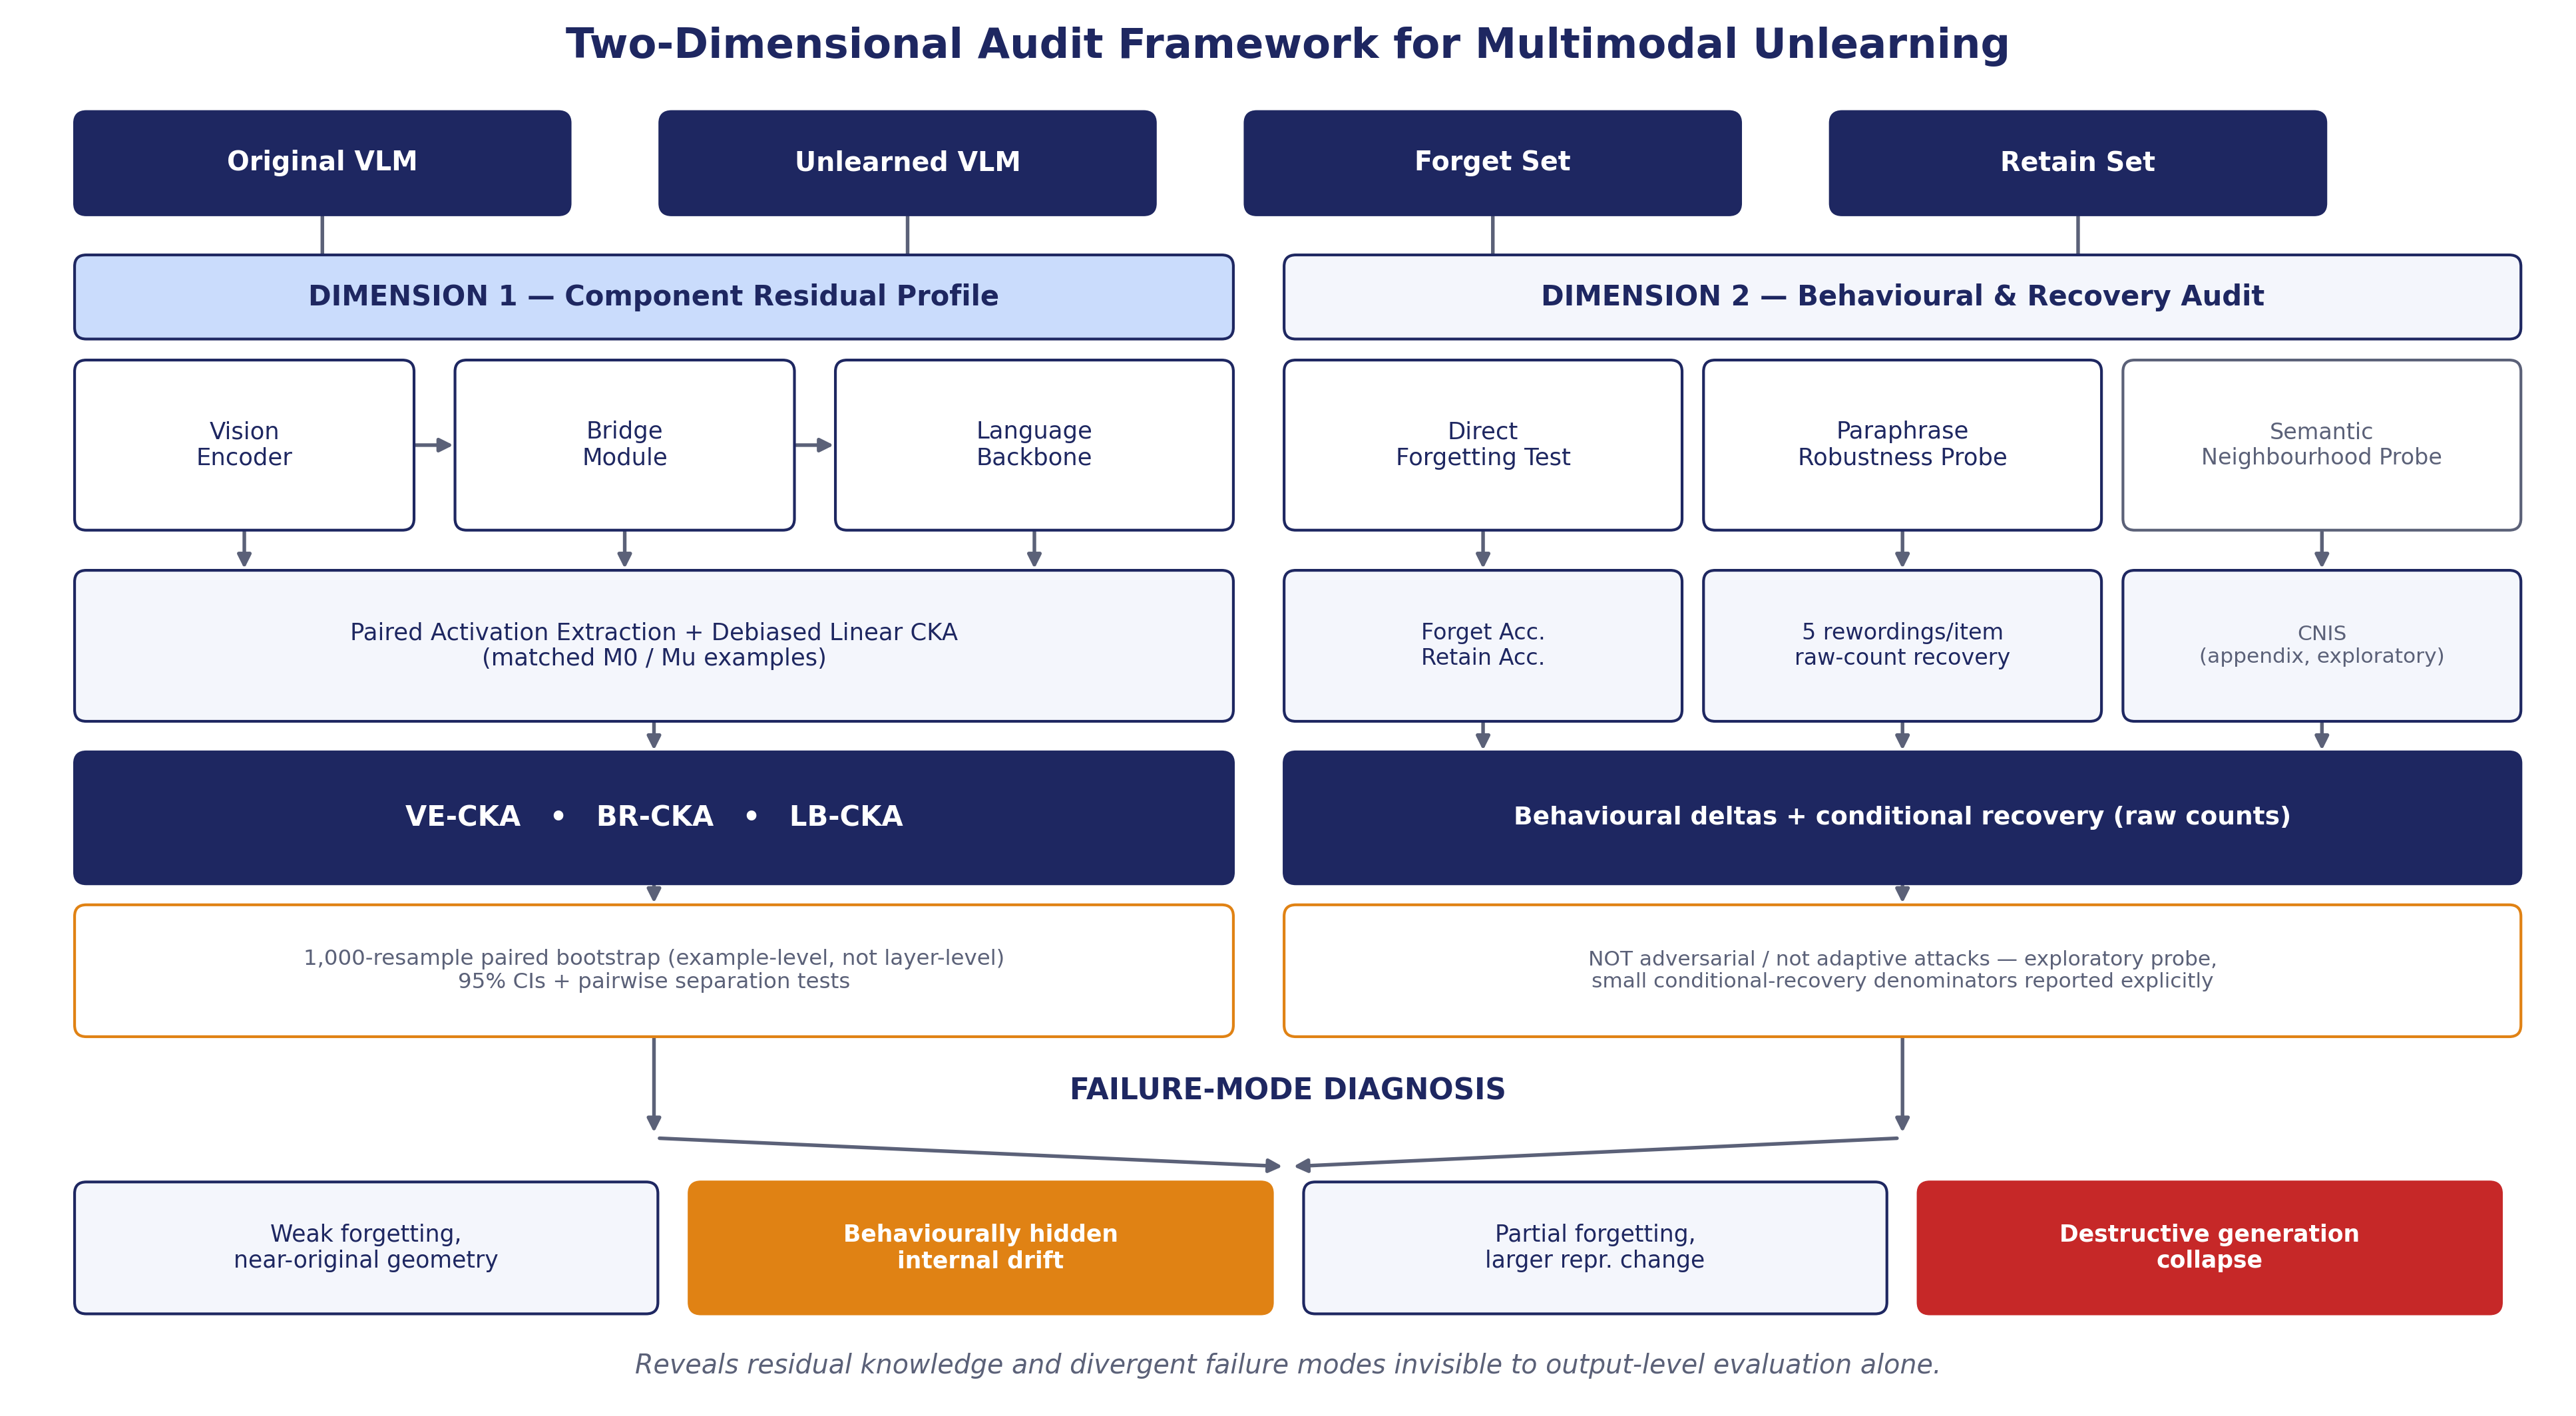
\includegraphics[width=\textwidth]{Figures/fig_framework.pdf}
\caption{Audit setup. The original and unlearned VLMs are compared on
forget and retain data. We measure CKA similarity inside the model and
report it with direct forgetting, recovery probing, retain utility, and
semantic-neighbourhood behaviour.}
\label{fig:framework}
\end{figure*}

Vision--language models (VLMs) are trained on large image--text datasets.
Some examples may later need to be removed because of privacy, copyright,
or data-use restrictions. Machine unlearning studies how to reduce the
influence of such data without retraining from scratch
\citep{bourtoule2021machine}.

Most tests focus on the model's output after unlearning: the model should
stop answering questions about the forgotten target while remaining accurate
on retain data \citep{liu2024mllmu,dontsov2024clear,ma2024fiubench}. This
test is useful, but it does not reveal what is happening inside the model. A
VLM has a vision encoder and a language backbone connected by a bridge, such
as an MLP projector or Q-Former. If the final answer is suppressed, residual
structure may remain in these components. The opposite can also occur: a
method may change the model too much and degrade retain utility. Output-only
evaluation therefore cannot reliably separate under-forgetting from
over-disruption \citep{liang2023helm}.

We study this problem with a two-dimensional audit framework. The first
dimension computes a Component Residual Profile (CRP) by applying debiased
linear CKA \citep{kornblith2019cka,nguyen2021dkcka} to stacked activation
matrices collected from the vision encoder, bridge, and language backbone of
the original model $\mathcal{M}_0$ and unlearned model $\mathcal{M}_u$. The
second dimension probes semantic-neighbourhood behaviour using the Concept
Neighborhood Integrity Score (CNIS), a Wikidata-grounded probe
\citep{vrandevcic2014wikidata}.

We evaluate LLaVA-1.5-7B \citep{liu2023llava} and BLIP-2-OPT-2.7B
\citep{li2023blip2} using five LoRA-based methods plus MANU across two MLLMU
splits, with independent validation on UnLOK-VQA \citep{patil2025unlok}.

Our contributions are as follows.
\textbf{(1)} We propose a two-dimensional audit framework for multimodal
unlearning that combines component-level representation analysis with
behavioural and semantic-neighbourhood probes.
\textbf{(2)} We introduce CRP, which localises residual similarity across the
vision encoder, multimodal bridge, and language backbone using matrix-level
debiased linear CKA on stacked forward-pass activation matrices.
\textbf{(3)} We introduce CNIS, a Wikidata-grounded
semantic-neighbourhood consistency probe.
\textbf{(4)} A GA schedule-sensitivity analysis reveals a progression from
under-forgetting through hidden internal drift to full collapse, demonstrating
that output metrics can remain unchanged while Bridge-CKA has already fallen
substantially.
\textbf{(5)} A projector-adaptation ablation provides a directional sensitivity
check for the bridge component, and an independent UnLOK-VQA evaluation shows
that similar output-level profiles can conceal substantially different
language-backbone geometries.

\section{Related Work}

\paragraph{Machine unlearning and evaluation.}
Machine unlearning reduces the influence of data after deployment
\citep{bourtoule2021machine}. MUSE shows that output-level checks are
insufficient for language models \citep{shi2024muse}. We extend this
evaluation view to multimodal unlearning.

\paragraph{Multimodal unlearning benchmarks.}
MLLMU-Bench \citep{liu2024mllmu}, CLEAR \citep{dontsov2024clear}, FIUBench
\citep{ma2024fiubench}, and UnLOK-VQA \citep{patil2025unlok} benchmark
multimodal unlearning; UnLOK-VQA adds adversarial paraphrase evaluation. These
benchmarks primarily judge models from outputs. Table~\ref{tab:coverage}
summarises coverage. Our CRP/CNIS audit is complementary rather than a
replacement.

\paragraph{Representation and knowledge localisation.}
CKA measures representational geometry similarity
\citep{kornblith2019cka,nguyen2021dkcka}. SVCCA is an alternative
\citep{raghu2017svcca}. Our CRP audit is distinct from causal tracing
\citep{meng2022rome,meng2023memit} and model editing \citep{mitchell2022serac},
which locate or modify factual associations rather than audit
representational residuals.

\paragraph{Broader evaluation context.}
Earlier unlearning work studied exact and approximate methods
\citep{cao2015towards,guo2020certified,golatkar2020eternal,wu2020deltagrad}.
HELM and VHELM show that benchmark design reveals model gaps
\citep{liang2023helm,lee2024vhelm}. Our work applies this perspective to
multimodal unlearning, building on PIQA \citep{bisk2020piqa}, calibration
methods \citep{lyu2025calibrating}, and structured VLM prompting
\citep{wang2024hpt}.

\section{Audit Framework}

The audit takes four inputs: the original VLM $\mathcal{M}_0$, the unlearned
VLM $\mathcal{M}_u$, a forget set $\mathcal{F}$, and a retain set
$\mathcal{R}$.

\subsection{Component-Level Residual Audit}

\paragraph{What CKA tells us.}
CKA is a diagnostic signal. High CKA means that a component's
representational geometry changed little; low CKA means stronger change, not
necessarily clean selective erasure. We therefore interpret CRP jointly with
retain utility, recovery evidence, and CNIS.

\paragraph{How activations are collected.}
We register forward hooks in the vision encoder, multimodal bridge, and
language backbone (Table~\ref{tab:hooks}). For each sample in $\mathcal{F}$,
we run a single forward pass through $\mathcal{M}_0$ and $\mathcal{M}_u$ and
collect mean-pooled hidden states at each hook. Vision and bridge activations
are mean-pooled over visual or query tokens; language-backbone activations are
mean-pooled over non-padding tokens. Because token content can differ between
models, LB-CKA is interpreted as a relative diagnostic signal.

\begin{table}[t]
\centering
\caption{Hook and aggregation protocol for component-level auditing.}
\label{tab:hooks}
\setlength{\tabcolsep}{4pt}
\scriptsize
\begin{tabular}{llll}
\toprule
\textbf{Component} & \textbf{LLaVA} & \textbf{BLIP-2} & \textbf{Pooling} \\
\midrule
Vision   & ViT      & EVA/CLIP & mean token \\
Bridge   & MLP      & Q-Former & mean query/token \\
Language & Vicuna   & OPT      & mean non-pad token \\
\bottomrule
\end{tabular}
\end{table}

\paragraph{CKA computation.}
The per-sample activation vectors are stacked across all $n$ forget-set
samples into matrices $\mathbf{X},\mathbf{Y}\in\mathbb{R}^{n\times d}$ for
$\mathcal{M}_0$ and $\mathcal{M}_u$ at the same hook. We compute
mean-centred, debiased linear CKA
\citep{kornblith2019cka,nguyen2021dkcka} on these matrices. A higher value
means that the unlearned model preserves more of the original component
geometry. Hook-level scores are averaged within each component to obtain
VE-CKA, Bridge-CKA, and LB-CKA, which together form the CRP.

\paragraph{Frozen components and interpretation.}
For attention-only HF-LoRA methods, adapters are attached to language-backbone
attention projections; no adapters are attached to the vision encoder or
bridge. In principle, matched deterministic evaluations of truly identical
frozen upstream modules should produce highly similar upstream activations.
Accordingly, unexpectedly low frozen-component CKA can also reflect
quantisation, separate model loading, hook placement, or activation-extraction
variability. We therefore treat absolute frozen-component values cautiously
and use the projector-adaptation ablation primarily as a directional check.

\subsection{Behavioural and Semantic Audit}

\paragraph{Direct forgetting and retain utility.}
Direct forgetting measures whether $\mathcal{M}_u$ still answers forget-set
queries. Retain utility measures accuracy on $\mathcal{R}$.

\paragraph{Recovery probing.}
We test whether forgotten information can be recovered through rephrased
textual prompts, centre-crop visual prompts, and Gaussian-noise perturbations.
A recovery case is counted when the response matches the target or an accepted
alias.

\paragraph{Concept Neighborhood Integrity Score.}
For each forget entity $e$, we fetch one-hop Wikidata neighbours
$N(e)$ \citep{vrandevcic2014wikidata} through a filtered relation set
(employer, collaborator, field of work, award received, educated at,
affiliated organisation, member of, notable work, co-author, related person).
For each neighbour $v\in N(e)$:
\begin{equation}
q(v)=
\begin{cases}
1,   & \text{exact or alias match},\\
0.5, & \text{partial string match},\\
0,   & \text{otherwise}.
\end{cases}
\end{equation}
\begin{equation}
\mathrm{CNIS}(e)=\frac{1}{|N(e)|}\sum_{v\in N(e)}q(v).
\end{equation}
CNIS is averaged over responsive entities with non-empty neighbourhoods and
marked N/R when retain utility collapses.

\section{Experimental Setup}

\subsection{Architectures}
LLaVA-1.5-7B \citep{liu2023llava} uses an MLP projector bridge;
BLIP-2-OPT-2.7B \citep{li2023blip2} uses a Q-Former. This pairing tests
whether unlearning behaviour depends on bridge design.

\subsection{Methods}
The LoRA-based methods are Gradient Ascent (GA), NPO, MMUnlearner, CAGUL,
and SineProject. In the LLaVA experiments, suffix-based attention targets
($q$, $k$, $v$, and $o$ projections) activate LoRA modules in both the
vision and language attention stacks; the multimodal projector remains
unchanged except in the controlled projector-adaptation ablation. GA uses
two checkpoint variants: a 50-step checkpoint (GA-attn4-50) for
\emph{mllmu\_real} CRP and schedule analysis, and a 20-step checkpoint
(GA-attn4-20) for UnLOK-VQA, where 50 steps causes behavioural collapse.
The audited LLaVA MANU adapter was inactive because its effective LoRA
updates were zero and is therefore excluded from LLaVA results. MANU is
retained only for BLIP-2, where checkpoint auditing confirmed active
updates.

\subsection{Benchmarks}
\textbf{mllmu\_real}: 20 forget entities ($n=40$ forget samples) and 40
retain entities ($n=80$ retain samples) representing real persons linked to
Wikidata. This split supports CNIS.

\textbf{mllmu\_bench}: 160 forget and 238 retain files with fictitious
personas. CNIS is not computed. Only methods backed by valid checkpoints are
reported for this auxiliary split.

\textbf{UnLOK-VQA} \citep{patil2025unlok}: 100 forget samples and 400
locality samples drawn from the benchmark. Built-in paraphrase queries serve
as recovery probes and provide independent validation on a different data
source.

\section{Results}

\subsection{Evaluation Coverage}

Table~\ref{tab:coverage} compares evaluation dimensions across frameworks.
It is a coverage summary, not a performance comparison.

\begin{table}[t]
\centering
\caption{Evaluation dimensions supported by multimodal unlearning frameworks.}
\label{tab:coverage}
\setlength{\tabcolsep}{4pt}
\footnotesize
\begin{tabular}{lcccc}
\toprule
\textbf{Dimension}     & \textbf{MLLMU} & \textbf{CLEAR} & \textbf{FIU} & \textbf{Ours} \\
\midrule
Output forgetting      & $\checkmark$ & $\checkmark$ & $\checkmark$ & $\checkmark$ \\
Retain utility         & $\checkmark$ & $\checkmark$ & $\checkmark$ & $\checkmark$ \\
Recovery probing       & $\times$     & $\times$     & $\circ$      & $\checkmark$ \\
Vision residual        & $\times$     & $\times$     & $\times$     & $\checkmark$ \\
Bridge residual        & $\times$     & $\times$     & $\times$     & $\checkmark$ \\
Language residual      & $\times$     & $\times$     & $\times$     & $\checkmark$ \\
Semantic consistency   & $\times$     & $\times$     & $\times$     & $\checkmark$ \\
Architecture diagnosis & $\times$     & $\times$     & $\times$     & $\checkmark$ \\
\bottomrule
\multicolumn{5}{l}{\footnotesize $\checkmark$ = supported; $\circ$ = partial;
$\times$ = not evaluated.}
\end{tabular}
\end{table}

\subsection{Component Residual Profile: LLaVA on \emph{mllmu\_real}}

Table~\ref{tab:crp_main} reports CRP for five LoRA-based methods on
\emph{mllmu\_real} using matrix-level debiased linear CKA on stacked
activation matrices.

\begin{table}[t]
\centering
\caption{Component Residual Profile on \emph{mllmu\_real}
(LLaVA-1.5-7B, $n=40$ forget samples). Values are mean debiased linear
CKA between stacked base-model and unlearned-model activation matrices.}
\label{tab:crp_main}
\setlength{\tabcolsep}{5pt}
\small
\begin{tabular}{lrrr}
\toprule
\textbf{Method} & \textbf{VE-CKA} & \textbf{BR-CKA} & \textbf{LB-CKA} \\
\midrule
GA-attn4-50 & 0.9235 & 0.5795 & 0.5333 \\
NPO         & 0.9997 & 0.9986 & 0.9931 \\
MMUnlearner & 0.9998 & 0.9965 & 0.9336 \\
CAGUL       & 0.9997 & 0.9973 & 0.9927 \\
SineProject & 0.9999 & 0.9986 & 0.9980 \\
\bottomrule
\end{tabular}
\end{table}

NPO, CAGUL, and SineProject remain nearly identical to the original model
across the three audited components. MMUnlearner preserves the vision encoder
and bridge but shows a moderate language-backbone shift
($\mathrm{LB\mbox{-}CKA}=0.934$). GA-attn4-50 differs substantially, with
Bridge-CKA $=0.580$ and LB-CKA $=0.533$. The spread in LB-CKA, from
$0.533$ to $0.998$, shows that methods with the same adapter scope can have
very different representational effects. Because the frozen-component values
for GA are unexpectedly low, we interpret those absolute VE and bridge values
cautiously and examine optimization-scope sensitivity separately.

\begin{figure}[t]
\centering
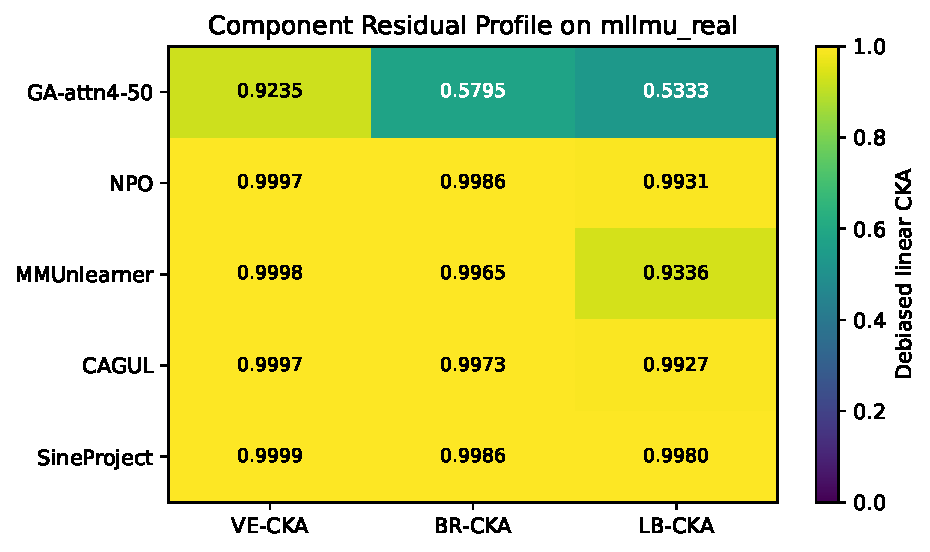
\includegraphics[width=\columnwidth]{Figures/fig_crp_heatmap.pdf}
\caption{CRP heatmap on \emph{mllmu\_real} using the validated
LLaVA results in Table~\ref{tab:crp_main}. The inactive LLaVA MANU adapter
is excluded.}
\label{fig:crp_heatmap}
\end{figure}

\subsection{GA Schedule Sensitivity}

To examine how training duration interacts with CRP, we evaluate GA-attn4 at
5, 10, 20, and 50 steps (Table~\ref{tab:schedule}).

\begin{table}[t]
\centering
\caption{Schedule sensitivity of attention-only GA on \emph{mllmu\_real}
(LLaVA-1.5-7B). At 5--10 steps, GA remains behaviourally
under-forgetting despite increasing internal drift. At 20 steps, retain
utility begins to deteriorate, while the 50-step schedule collapses
generation.}
\label{tab:schedule}
\setlength{\tabcolsep}{3pt}
\small
\begin{tabular}{rrrrrrr}
\toprule
\textbf{Steps} & \textbf{F-Acc}$\downarrow$ & \textbf{F-Rate}$\uparrow$
& \textbf{Ret-Acc}$\uparrow$ & \textbf{VE-CKA} & \textbf{BR-CKA}
& \textbf{LB-CKA} \\
\midrule
 5 & 0.9750 & 0.0250 & 0.9625 & 0.9927 & 0.9337 & 0.8934 \\
10 & 0.9750 & 0.0250 & 0.9750 & 0.9845 & 0.8079 & 0.7299 \\
20 & 0.9250 & 0.0750 & 0.8750 & 0.9557 & 0.5260 & 0.4828 \\
50 & 0.0000 & 1.0000 & 0.0000 & 0.9235 & 0.5795 & 0.5333 \\
\bottomrule
\end{tabular}
\end{table}

At 5 steps, GA barely forgets and internal change is limited. At 10 steps,
output behaviour is unchanged relative to 5 steps (Forget Rate $=0.025$),
yet Bridge-CKA falls to $0.808$ and LB-CKA to $0.730$. This exposes
substantial internal drift before the output metric changes. At 20 steps,
forgetting remains weak while retain accuracy decreases to $0.875$,
indicating growing over-disruption. At 50 steps, both forget and retain
accuracy collapse to zero. The resulting F-Rate of $1.000$ therefore does not constitute selective unlearning. The sequence from under-forgetting to hidden
internal drift, utility degradation, and full collapse becomes visible only
when behavioural and internal evidence are considered together.

\subsection{Controlled Projector-Adaptation Ablation}

To verify that Bridge-CKA responds to direct projector updates, we compare
two matched 50-step GA conditions. Both use the same LoRA rank, optimisation
schedule, data, and vision--language attention targets. The second condition
adds LoRA only to the two multimodal-projector linear layers
(Table~\ref{tab:bridge_ablation}).

\begin{table}[t]
\centering
\caption{Controlled projector-adaptation ablation for LLaVA-1.5-7B using
GA. Both conditions apply LoRA to vision and language attention modules;
the projector-adapted condition additionally applies LoRA to the multimodal
MLP projector.}
\label{tab:bridge_ablation}
\setlength{\tabcolsep}{5pt}
\small
\begin{tabular}{lrrr}
\toprule
\textbf{Setting} & \textbf{VE-CKA} & \textbf{BR-CKA} & \textbf{LB-CKA} \\
\midrule
GA-attn4-50 (frozen projector) & 0.9973 & 0.9910 & 0.8987 \\
GA-attn4-50 (projector adapted) & 0.9789 & 0.9024 & 0.2260 \\
\bottomrule
\end{tabular}
\end{table}

Direct projector adaptation reduces Bridge-CKA from $0.991$ to $0.902$,
confirming that the bridge component of CRP responds to actual projector
updates. VE-CKA remains comparatively high ($0.979$), whereas LB-CKA falls
to $0.226$. This experiment is a controlled sensitivity test: the only
target-scope difference is the addition of projector LoRA, with no language
feed-forward adapters enabled.

\subsection{Behavioural and Semantic Controls}

\paragraph{Output-level results.}
NPO, MMUnlearner, CAGUL, and SineProject retain high utility
($0.963$--$0.975$) but show almost no direct forgetting: forget accuracy
remains $0.975$, matching the no-unlearn baseline. For the methods evaluated
in Table~\ref{tab:recovery}, adversarial recovery also remains high
($0.875$--$0.887$). Together with Table~\ref{tab:crp_main}, these results
support an under-forgetting diagnosis for the evaluated LoRA methods.

\begin{table}[t]
\centering
\caption{Adversarial recovery on \emph{mllmu\_real} (LLaVA-1.5-7B).
Direct $=$ identity query; Rephrase $=$ paraphrase without entity name;
Crop $=$ centre crop at $0.6\times$; Perturb $=$ Gaussian noise
$\sigma=25$.}
\label{tab:recovery}
\setlength{\tabcolsep}{4pt}
\small
\begin{tabular}{lrrrrr}
\toprule
\textbf{Method} & \textbf{Direct} & \textbf{Reph.}
& \textbf{Crop} & \textbf{Perturb} & \textbf{Mean} \\
\midrule
NPO         & 0.975 & 0.850 & 0.700 & 0.975 & 0.875 \\
MMUnlearner & 0.975 & 0.875 & 0.725 & 0.975 & 0.887 \\
CAGUL       & 0.975 & 0.850 & 0.700 & 0.975 & 0.875 \\
\bottomrule
\end{tabular}
\end{table}

The inactive LLaVA MANU adapter is excluded from this recovery comparison.
No behavioural value from that checkpoint is treated as an unlearning
result.

\paragraph{CNIS baseline.}
The original model gives CNIS $=0.870$ on the 20 forget-set entities. After
unlearning, NPO ($0.872$), MMUnlearner ($0.869$), and CAGUL ($0.858$)
remain close to this value. A shuffled-relation control
(Appendix~\ref{app:cnis}) gives $0.844$, a gap of $0.046$. We interpret CNIS
as a semantic consistency probe rather than a leakage detector. No GA CNIS
value is reported because the previously available GA result came from the
invalid adapter configuration.

\begin{figure}[t]
\centering
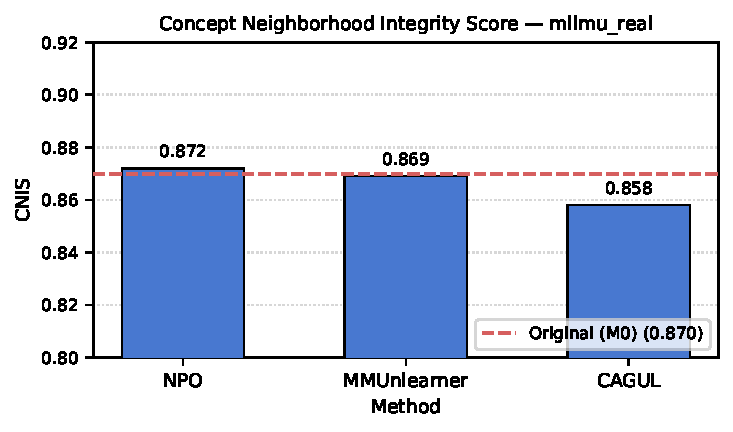
\includegraphics[width=\columnwidth]{Figures/fig_cnis.pdf}
\caption{CNIS on \emph{mllmu\_real}. NPO, MMUnlearner, and CAGUL remain
close to the original-model baseline ($0.870$). MANU is non-interpretable
because retain utility collapses. No GA value is included.}
\label{fig:cnis}
\end{figure}

\subsection{Cross-Architecture Analysis: BLIP-2}

Table~\ref{tab:blip2} reports the BLIP-2 CRP. Gradient-based methods keep
VE-CKA and Bridge-CKA at $1.000$, consistent with frozen Q-Former and vision
modules. The language backbone separates the methods: GA and CAGUL remain
above $0.98$, whereas NPO and MMUnlearner fall to approximately $0.67$, with
divergence localised to layer 6 (NPO: $0.088$; MMUnlearner: $0.100$).
Table~\ref{tab:blip2_behavioral} shows identical output behaviour for all
adapters (ForgetAcc $=0.400$, RetainAcc $=0.288$). This provides a
within-architecture example of identical output profiles concealing different
internal geometries.

\begin{table}[t]
\centering
\caption{BLIP-2-OPT-2.7B CRP on \emph{mllmu\_real}. Behavioural results
are reported separately in Table~\ref{tab:blip2_behavioral}.}
\label{tab:blip2}
\setlength{\tabcolsep}{6pt}
\small
\begin{tabular}{lccc}
\toprule
\textbf{Method} & \textbf{VE-CKA} & \textbf{BR-CKA} & \textbf{LB-CKA} \\
\midrule
GA          & 1.000 & 1.000 & 0.9945 \\
NPO         & 1.000 & 1.000 & 0.6699 \\
MMUn.       & 1.000 & 1.000 & 0.6721 \\
CAGUL       & 1.000 & 1.000 & 0.9834 \\
\midrule
MANU        & 0.5753 & 0.3157 & 0.5286 \\
\bottomrule
\end{tabular}
\end{table}

\begin{table}[t]
\centering
\caption{BLIP-2 behavioural results. All adapters match the no-unlearn
baseline; results are interpreted only as within-architecture comparisons.}
\label{tab:blip2_behavioral}
\setlength{\tabcolsep}{5pt}
\footnotesize
\begin{tabular}{lrrrr}
\toprule
\textbf{Method}
& \textbf{F-Acc}$\downarrow$ & \textbf{F-Rate}$\uparrow$
& \textbf{Ret-Acc} & \textbf{LB-CKA} \\
\midrule
No-unl. & 0.400 & 0.600 & 0.288 & 1.000 \\
\midrule
GA      & 0.400 & 0.600 & 0.288 & 0.995 \\
NPO     & 0.400 & 0.600 & 0.288 & 0.670 \\
MMUn.   & 0.400 & 0.600 & 0.288 & 0.672 \\
CAGUL   & 0.400 & 0.600 & 0.288 & 0.983 \\
MANU    & 0.400 & 0.600 & 0.288 & 0.529 \\
\bottomrule
\end{tabular}
\end{table}

\begin{figure}[t]
\centering
\includegraphics[width=\columnwidth]{Figures/fig_cross_arch.pdf}
\caption{Cross-architecture CRP. MANU shows strong representational
disruption in the architectural-audit implementation. Its results are not
directly combined with the LoRA behavioural columns because the available
implementations are unmatched.}
\label{fig:cross_arch}
\end{figure}

\subsection{Independent Validation: UnLOK-VQA}

Table~\ref{tab:unlok_full} reports results on the UnLOK-VQA subset
($n=100$ forget and $n=400$ locality samples).

\begin{table}[t]
\centering
\caption{Audit on an \emph{UnLOK-VQA} subset using LLaVA-1.5-7B
($n=100$ forget and $n=400$ locality samples). Rephrase denotes recovery
under built-in paraphrased queries. CRP values use debiased linear CKA.}
\label{tab:unlok_full}
\setlength{\tabcolsep}{3pt}
\small
\begin{tabular}{lrrrrrr}
\toprule
\textbf{Method} & \textbf{F-Acc}$\downarrow$
& \textbf{Ret-Acc}$\uparrow$ & \textbf{Reph.}$\downarrow$
& \textbf{VE-CKA} & \textbf{BR-CKA} & \textbf{LB-CKA} \\
\midrule
GA-attn4-20 & 0.680 & 0.820 & 0.588 & 0.998 & 0.977 & 0.772 \\
NPO         & 0.680 & 0.860 & 0.593 & 1.000 & 1.000 & 1.000 \\
MMUnlearner & 0.690 & 0.853 & 0.571 & 1.000 & 0.999 & 0.957 \\
CAGUL       & 0.680 & 0.863 & 0.591 & 1.000 & 1.000 & 1.000 \\
SineProject & 0.690 & 0.863 & 0.586 & 1.000 & 1.000 & 0.999 \\
\bottomrule
\end{tabular}
\end{table}

Forget-set accuracy lies between $0.680$ and $0.690$ for all five methods,
indicating under-forgetting. Retain accuracy remains reasonably high and
paraphrase recovery rates are similar ($0.571$--$0.593$). Despite this
behavioural similarity, the language-backbone geometries differ:
GA-attn4-20 has LB-CKA $=0.772$, MMUnlearner has LB-CKA $=0.957$, and NPO,
CAGUL, and SineProject remain approximately $1.000$. This independently
supports the central claim that similar output-level forgetting can conceal
different internal representational changes.

\subsection{Cross-Dataset Validation}

The auxiliary \emph{mllmu\_bench} split is reported only for MMUnlearner.
No valid recomputed GA result exists for this split, and the inactive LLaVA
MANU adapter is excluded. MMUnlearner retains high utility while showing a
language-backbone shift. The result is provided in
Appendix~\ref{app:bench}; no claim is made for GA or MANU on this auxiliary
LLaVA split.

\subsection{Additional Diagnostic Controls}

Appendix~\ref{app:e7controls} reports controls for extraction stability,
forget--retain selectivity, layerwise localisation, and update magnitude.
A same-configuration base-vs-base comparison gives CKA $=1.0000$ at all
reported hooks from \texttt{ve\_6} through \texttt{ve\_23}, the bridge, and
\texttt{lb\_0} through \texttt{lb\_31}. NPO shows a positive forget--retain
selectivity gap at all five sampled language layers. MMUnlearner instead
shows retained-set damage at L31, while GA causes broad disruption under
complete behavioural collapse. Effective LoRA update norms explain much of
the pooled CKA variation, but the final language layer remains more sensitive
than update magnitude alone predicts.

\section{Limitations}

\textbf{CKA robustness.}
Activation matrices were not retained after extraction, so SVCCA, PWCCA,
token-aligned comparisons, and pooling-sensitivity controls require a
dedicated re-extraction pipeline. CKA is a diagnostic probe, not causal
evidence of knowledge removal. The LLaVA per-layer analysis is available for
NPO, MMUnlearner, CAGUL, and SineProject, but not for GA-attn4-50.

\textbf{Representation-extraction reproducibility.}
The base-vs-base control yields CKA $=1.0000$ at all reported hooks from
\texttt{ve\_6} through \texttt{ve\_23}, the bridge, and
\texttt{lb\_0} through \texttt{lb\_31}, supporting deterministic extraction
for those hooks under the tested configuration. The controlled projector
ablation uses matched hook resolution and evaluation settings and therefore
supersedes the earlier confounded comparison. Full-precision replication and
additional pooling or token-alignment controls remain future work.

\textbf{Training schedule.}
The schedule-sensitivity analysis shows that regime assignment depends on
step count. Our primary evaluations use method-appropriate schedules, but
exhaustive hyperparameter sweeps are beyond the current scope. The
under-forgetting of NPO, CAGUL, and SineProject may partly reflect
insufficient optimisation.

\textbf{Semantic consistency probe.}
High CNIS may indicate preserved semantic utility or residual associative
access. We interpret CNIS jointly with all other signals. The exact inclusion
count for the main CNIS evaluation remains unverified and is therefore not
reported; the 17-entity count in Appendix~\ref{app:cnis} applies only to the
shuffled-relation control. CNIS confidence intervals and a human-judged
verification subset are also not yet available.

\textbf{Recovery scope.}
The recovery audit uses direct, rephrased, cropped, and perturbed queries.
Stronger adaptive black-box search, white-box recovery attacks, and
retraining-based recovery remain future work.

\textbf{Bridge hypothesis.}
BLIP-2 Bridge-CKA equals $1.000$ for gradient-based methods because the
Q-Former is frozen under the tested HF-LoRA setup. The bridge-unfreeze
ablation was performed on LLaVA only. Whether the Q-Former behaves similarly
under direct adaptation remains open.

\textbf{MANU validity.}
Checkpoint auditing showed that the available LLaVA MANU adapter had zero
effective LoRA updates, so it is excluded from all LLaVA comparisons. The
BLIP-2 MANU checkpoint was active and is retained only in the corresponding
BLIP-2 analysis.

\textbf{Oracle and bridge controls.}
We do not compare CRP with a retain-only retraining oracle or a
distance-to-oracle metric, and we do not report a trainable Q-Former ablation
for BLIP-2. These controls would help calibrate whether lower CRP corresponds
to desirable selective removal rather than generic disruption.

\textbf{Entity set and quantisation.}
The \emph{mllmu\_real} analysis uses 20 entities and 4-bit NF4 quantisation.
Larger entity sets and full-precision runs are needed for stronger
statistical claims.

\section{Conclusion}

We presented a framework for evaluating multimodal machine unlearning beyond
final outputs by combining CRP with CNIS. Across two VLM architectures, two
MLLMU splits, five LoRA-based methods plus MANU, and independent UnLOK-VQA
validation, methods with similar output-level forgetting profiles exhibit
substantially different internal representational changes. NPO, CAGUL, and
SineProject remain near the original model internally, whereas MMUnlearner
shows moderate language-backbone drift. A GA schedule-sensitivity analysis reveals hidden
internal drift before output forgetting changes and complete behavioural
collapse at 50 steps. A controlled projector-adaptation ablation reduces
Bridge-CKA from $0.991$ to $0.902$, showing that the bridge metric responds
to direct projector updates. Retain-set and layerwise controls distinguish
selective change from collateral damage: NPO is weakly but consistently
selective, MMUnlearner damages retained representations at L31, and GA causes
broad disruption. Effective update magnitude explains much of the overall
drift, but not the disproportionate sensitivity of the terminal language
layer. These findings support evaluating multimodal unlearning through
behavioural, component-level, semantic-neighbourhood, and checkpoint-validity
evidence.

\bibliography{aaai2027}

\clearpage
\appendix

\section{Additional Controls and Validation}

\subsection{Testing on \emph{mllmu\_bench}}
\label{app:bench}

No valid recomputed GA checkpoint result is available for this auxiliary
split, so GA is omitted. The available LLaVA MANU adapter was inactive and
is also excluded. MMUnlearner retains high utility while changing the
language backbone. Bootstrap intervals are reported only for this valid
result.

\begin{table}[h]
\centering
\caption{Valid reported result on \emph{mllmu\_bench} with LLaVA.
GA is omitted because no valid recomputed checkpoint is available, and the
inactive LLaVA MANU adapter is excluded. CNIS is not reported for fictitious
personas.}
\label{tab:bench_appendix}
\setlength{\tabcolsep}{3pt}
\scriptsize
\begin{tabular}{lllll}
\toprule
\textbf{Method} & \textbf{VE-CKA} & \textbf{BR-CKA}
& \textbf{LB-CKA} & \textbf{Retain} \\
\midrule
MMUn.
& 0.9996 & 0.9976 & 0.7899 [.7787,.7995] & 0.9923 \\
\bottomrule
\end{tabular}
\end{table}


\subsection{Base-vs-Base, Retain-Set, and Layerwise Controls}
\label{app:e7controls}

\paragraph{Base-vs-base extraction control.}
Independently loaded copies of the same base checkpoint were evaluated with
the same extraction configuration. All reported hooks give CKA $=1.0000$
(Table~\ref{tab:base_vs_base}), establishing deterministic extraction at
those hooks. The \texttt{ve\_0} hook is absent from the reported output; it is
not yet clear whether the hook failed to fire, the activation was missing, or
the resulting CKA was filtered as invalid. The control therefore does not
resolve the low frozen-component values observed for GA-attn4-50.

\begin{table}[h]
\centering
\caption{Base-vs-base CKA under the tested extraction configuration.
\texttt{ve\_0} is unresolved and excluded.}
\label{tab:base_vs_base}
\setlength{\tabcolsep}{7pt}
\scriptsize
\begin{tabular}{lr}
\toprule
\textbf{Hook} & \textbf{CKA} \\
\midrule
\texttt{ve\_6}  & 1.0000 \\
\texttt{ve\_12} & 1.0000 \\
\texttt{ve\_18} & 1.0000 \\
\texttt{ve\_23} & 1.0000 \\
\texttt{bridge} & 1.0000 \\
\texttt{lb\_0}  & 1.0000 \\
\texttt{lb\_8}  & 1.0000 \\
\texttt{lb\_16} & 1.0000 \\
\texttt{lb\_24} & 1.0000 \\
\texttt{lb\_31} & 1.0000 \\
\bottomrule
\end{tabular}
\end{table}

\paragraph{Retain-set CRP and selectivity.}
Table~\ref{tab:selectivity} compares forget-set and retain-set CRP. The
selectivity gap is defined as retain LB-CKA minus forget LB-CKA, so a positive
value denotes greater forget-side representational change. NPO, CAGUL, and
SineProject show negligible gaps and remain near the original model on both
sets. MMUnlearner has a small negative gap, indicating slightly greater
retain-side change. GA-attn4-50 has the largest positive gap, but it also has
zero forget and retain accuracy at 50 steps; this is over-disruption under collapse rather than selective unlearning.

\begin{table*}[h]
\centering
\caption{Forget-set and retain-set CRP on \emph{mllmu\_real}. The gap is
$\mathrm{R\mbox{-}LB}-\mathrm{F\mbox{-}LB}$; positive values indicate
greater forget-side change.}
\label{tab:selectivity}
\setlength{\tabcolsep}{4pt}
\scriptsize
\begin{tabular}{lrrrrrrr}
\toprule
\textbf{Method} & \textbf{F-VE} & \textbf{R-VE}
& \textbf{F-BR} & \textbf{R-BR}
& \textbf{F-LB} & \textbf{R-LB} & \textbf{Gap} \\
\midrule
NPO         & 0.9997 & 0.9998 & 0.9986 & 0.9992 & 0.9931 & 0.9972 & +0.004 \\
MMUnlearner & 0.9998 & 0.9999 & 0.9965 & 0.9982 & 0.9336 & 0.9269 & -0.007 \\
CAGUL       & 0.9997 & 0.9999 & 0.9973 & 0.9990 & 0.9927 & 0.9957 & +0.003 \\
SineProject & 0.9999 & 1.0000 & 0.9986 & 0.9995 & 0.9980 & 0.9991 & +0.001 \\
GA-attn4-50 & 0.9235 & 0.9605 & 0.5795 & 0.7926 & 0.5333 & 0.6318 & +0.098 \\
\bottomrule
\end{tabular}
\end{table*}

\paragraph{LLaVA per-layer language-backbone CKA.}
For the four methods with available data, CKA remains high from L0 through
L24 and shows its largest reduction at L31 (Table~\ref{tab:lb_per_layer}).
MMUnlearner has the strongest final-layer drop. This complements the BLIP-2
layer-localisation result but does not replicate it exactly because the
architectures and sampled layer positions differ. GA-attn4-50 is omitted
because its current JSON output does not contain valid per-layer values.

\begin{table}[h]
\centering
\caption{Per-layer LLaVA language-backbone CKA. GA-attn4-50 is unavailable
from the current output files.}
\label{tab:lb_per_layer}
\setlength{\tabcolsep}{4pt}
\scriptsize
\begin{tabular}{lrrrrr}
\toprule
\textbf{Method} & \textbf{L0} & \textbf{L8} & \textbf{L16}
& \textbf{L24} & \textbf{L31} \\
\midrule
NPO         & 0.9986 & 0.9982 & 0.9980 & 0.9989 & 0.9721 \\
MMUnlearner & 0.9964 & 0.9959 & 0.9958 & 0.9916 & 0.6882 \\
CAGUL       & 0.9973 & 0.9967 & 0.9967 & 0.9988 & 0.9742 \\
SineProject & 0.9986 & 0.9983 & 0.9985 & 0.9994 & 0.9951 \\
\bottomrule
\end{tabular}
\end{table}

\subsection{CNIS Specificity Control}
\label{app:cnis}

The original-model CNIS is $0.870$. A shuffled-relation control, in which
neighbour labels are permuted across relation prompts while model responses
are held fixed, produces $0.844$ across 17 entities with at least two valid
neighbours, a gap of $0.046$. This 17-entity count applies only to the
shuffled control and is not used as the main CNIS inclusion count. The modest
gap warrants a conservative interpretation. CNIS is therefore treated as a
consistency probe rather than a precise leakage measure.

\subsection{Prompt and Scoring Details}

Fixed greedy decoding is used throughout. Entity answers use exact, alias, and
normalised partial matching. CNIS prompts follow the template ``What is the
[relation] of [entity]?'' Answers are lowercased, punctuation-normalised, and
matched against Wikidata labels and aliases. Entities with empty or ambiguous
neighbourhoods are excluded; CNIS is marked N/R when retain utility collapses.

\subsection{Audit Reproduction Guide}

To reproduce CRP, hooks are registered at the vision encoder, bridge, and
language backbone following Table~\ref{tab:hooks}. A single forward pass is
run for each forget-set sample; hook outputs are mean-pooled and stacked
across all samples before CKA is computed. Each run stores a JSON summary with
component CKA, per-layer CKA when available, forget and retain accuracy,
recovery scores, and CNIS outputs. For frozen-component validation, future
runs should load the base and adapted models within the same process, enforce
identical preprocessing and quantisation settings, and include a base-vs-base
control for every audited hook.

\end{document}
